\documentclass{article}
\usepackage{graphicx}
\usepackage{xfrac}
\usepackage{../Ceyhun}
\usepackage{../amsTurkish}
\begin{document}
    \hPage{ceyhun-120} %page number
    yazabiliriz. Ayrıca, çizgenin düğüm kümesini $\Delta$ ile gösterirsek bu kesitlemeleri,
    \begin{center}
        $K_{1}=A(\Delta_{1}\times \bar\Delta_{1})=A(\Delta\times \Delta) \oplus A(\Delta_{1}\times \Delta_{1}) \oplus A(\bar\Delta_{1}\times \bar\Delta_{1})$\\
    \end{center}
    \begin{center}
        $K_{2}=A(\Delta_{2}\times \bar\Delta_{2})=A(\Delta\times \Delta) \oplus A(\Delta_{2}\times \Delta_{2}) \oplus A(\bar\Delta_{2}\times \bar\Delta_{2})$\\
    \end{center}
    biçiminde de yazabiliriz. $\Delta_{1}$ ve $\Delta_{2}$ nin,
    \begin{center}
        $\Delta_{1} = \Delta_{11} \cup \Delta_{12}$ 
    \end{center}
    \begin{center}
        $\bar\Delta_{2} = \Delta_{21} \cup \Delta_{22}$\\
    \end{center}
    \begin{center}
        $\Delta_{2} = \Delta_{11} \cup \Delta_{21}$\\
    \end{center}
    biçiminde altkümelere ayrıldığını düşünelim(Şekil 3.1.2). Öyleyse,
    
    \begin{figure}[h]
        \centering
        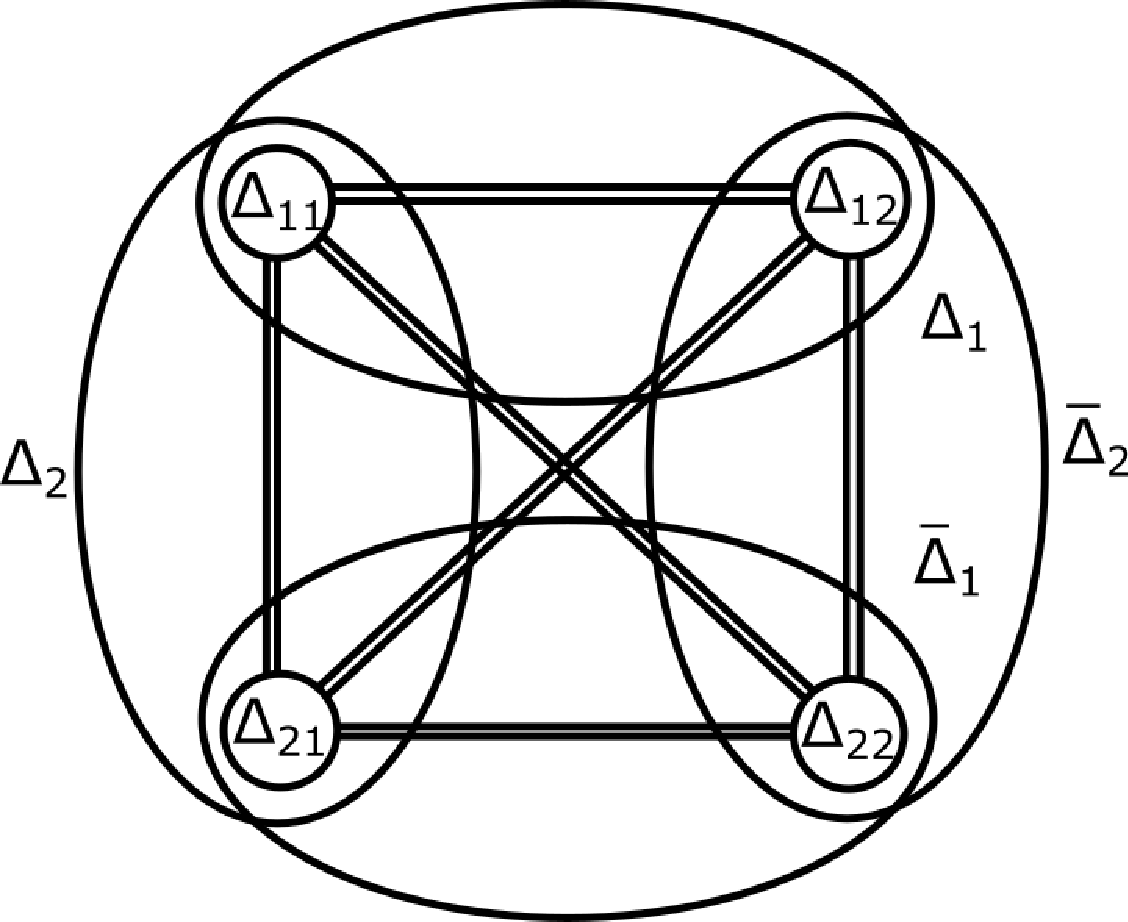
\includegraphics[width=0.6\textwidth]{images/ceyhun-120-fig01.pdf}
        \caption{Düğüm kümesinin dört altkümeye ayrılması.}
        \label{fig:drawing2}
    \end{figure}
\end{document}